\chapter{Antecedentes}\label{cap:estadodelarte}

\noindent Este segundo cap\'itulo pretende acercar al lector los conceptos clave que definen tanto  la computaci\'on cloud como el arquetipo MapReduce. Sobre ellos se apoyar\'an las elaboraciones posteriores relacionadas con el proyecto.


\section{Computaci\'on cloud}\label{sec:computacioncloud}
\noindent En esencia, el \emph{cloud computing}, computaci\'on cloud, o nube computacional, es un modelo de computaci\'on distribuida que pretende facilitar el consumo de esa infraestructura distribuida bajo la forma de recursos computacionales virtuales, plataformas virtuales o servicios. Sin embargo, no es una nueva tecnolog\'ia o arquitectura sino que representa un nuevo modo de explotaci\'on de recursos. Lo que se pretende con los cloud es flexibilizar la forma de dirigir el comportamiento de los centros de datos de cualquier tama\~no, de forma que un usuario pueda conformar computadores virtuales a su antojo (Infraestructura como Servicio o \emph{IaaS}), explotar un entorno de pruebas sobre un sistema operativo o plataforma software concretos (Plataforma como Servicio o \emph{PaaS}) o hacer uso de un servicio espec\'ifico como la copia de seguridad remota (Software como Servicio o \emph{SaaS}). La figura \ref{fig:cloudlayers} muestra el correspondiente diagrama de capas de alto nivel de un cloud gen\'erico.\newline

\begin{figure}[tbp]
\begin{center}
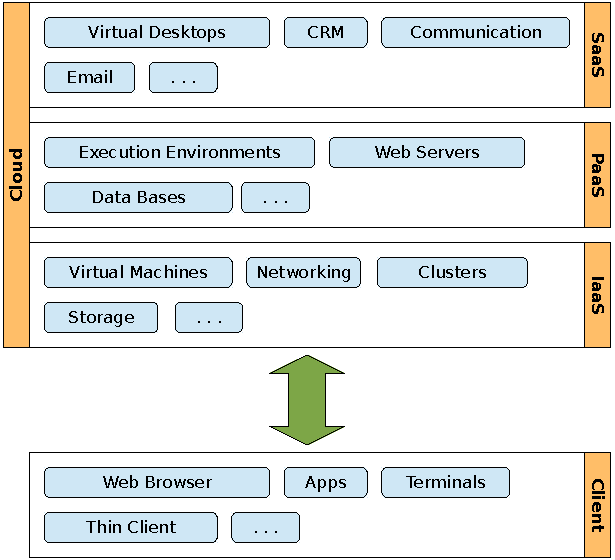
\includegraphics[width=0.69\textwidth]{imagenes/003.pdf}
 \caption{Capas de servicio de un cloud}
\label{fig:cloudlayers}
\end{center}
\end{figure}

Los distintos frameworks van a soportar la funcionalidad necesaria para manejar la infraestructura que defina al cloud. Ahora bien, ser\'a necesario un esfuerzo de an\'alisis, dise\~no, configuraci\'on, instalaci\'on y mantenimiento del servicio que se pretenda otorgar, teniendo en cuenta que el grado de elaboraci\'on de \'este aumenta desde los tipo IaaS hasta los tipo SaaS; efectivamente, las capas PaaS y SaaS se apoyan en sus respectivas capas soporte (IaaS para PaaS y PaaS para SaaS) que habr\'an de ser configuradas como se requiera. Todos los frameworks IaaS ---o, simplificadamente, herramientas de creaci\'on y mantenimiento de clouds para el manejo de m\'aquinas virtuales--- centran su atenci\'on en la configuraci\'on de un entorno estable definido por cuatro variables: CPUs virtuales, memoria de ejecuci\'on (RAM virtual), memoria de persistencia (HDD virtual) y redes virtuales. Este entorno de ejecuci\'on hace posible lanzar clusters virtuales completos sobre los que instalar plataformas o sistemas para ser posteriormente consumidos por usuarios; creando como efecto las capas software del cloud correspondientes ---PaaS y SaaS, respectivamente.\newline

Otras cuestiones no menos importantes, como el control de acceso, los permisos de ejecuci\'on, las cuotas o el almacenamiento persistente y seguro, tambi\'en tendr\'an representaci\'on en todos los frameworks.


\subsection{Arquitectura}\label{subsec:arquitecturacloud}
\noindent La figura \ref{fig:cloudlayers} mostraba las posibles capas que pueden formar parte del conjunto de servicios de un cloud en funcionamiento. En funci\'on de las capas implementadas, del framework concreto y del \emph{rol} que est\'e jugando el nodo del cl\'uster que ejecute un cloud, aparecer\'an asociados distintos \emph{m\'odulos} que hacen posible el consumo de los servicios configurados. Estos m\'odulos pueden concebirse como subsistemas de los cloud que conectan cada una de las partes necesarias para la ejecuci\'on de m\'aquinas virtuales, definidas fundamentalmente por las cuatro variables comentadas con anterioridad ---VCPUs, RAM, HDD y red. No existe una metodolog\'ia que dicte c\'omo han de ser estos subsistemas, en cuanto a tama\~no y responsabilidades, y as\'i, cada framework hace su propia partici\'on modular de la gesti\'on de infraestructura.\newline

Dejando de lado la modularidad, un concepto destacable de los cloud es la separaci\'on de responsabilidad en dos roles principales: \emph{Cloud Controller} y \emph{Cloud Node}. La figura \ref{fig:archcloud} muestra un despliegue gen\'erico de un cloud en un cl\'uster donde se han identificado ambos roles. La idea es seguir el modelo de las arquitecturas \emph{Maestro-Esclavo}.\newline

\begin{figure}[tbp]
\begin{center}
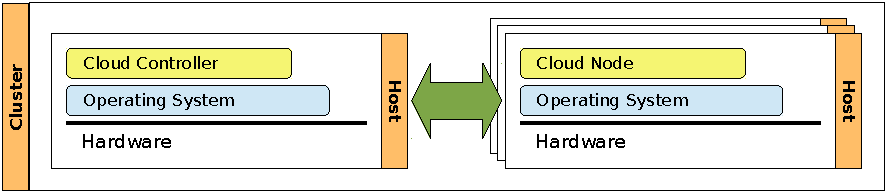
\includegraphics[width=0.9\textwidth]{imagenes/004.pdf}
 \caption{Controlador y nodo de un cloud}
\label{fig:archcloud}
\end{center}
\end{figure}

Dentro de esa distribuci\'on general, los anfitriones o nodos del cl\'uster ---ya sean \emph{controlador} o \emph{nodo} del cloud--- cooperan de forma sincronizada usando \emph{NTP} (\emph{Network Time Protocol}) y el paradigma \emph{paso de mensajes} implementado con colas de prioridad. Se basan adem\'as en la pol\'itica de \emph{nada compartido} para facilitar la escalabilidad. La estructura global de almacenamiento ---inherentemente compartida--- es una base de datos que corre, normalmente, en el controlador o controladores del cloud, o exclusivamente en un nodo del cl\'uster ---la base de datos asociada a un cloud es un ejemplo de un tipo de m\'odulo de persistencia. Un ordenador del cl\'uster puede hacer las veces de controlador y nodo al mismo tiempo, aunque bien es cierto que este \'ultimo apunte no est\'a recomendado fuera de \'ambitos de desarrollo por razones obvias.


\subsubsection{Cloud Controller}\label{subsubsec:cloudcontroller}
\noindent La tarea fundamental del nodo del cl\'uster designado como controlador es mantener el funcionamiento del cloud coordinando la cooperaci\'on de sus m\'odulos. Por ejemplo, algunas tareas de las que se encarga el controlador son las siguientes:

\begin{itemize}
 \item Control de autenticaci\'on y autorizaci\'on.
 \item Recuento de infraestructura f\'isica disponible.
 \item Control de cuotas de operaci\'on.
 \item Balance de consumo.
 \item Inventario de usuarios y proyectos.
 \item Exposici\'on del API para la explotaci\'on de los servicios.
 \item Monitorizaci\'on en tiempo real del cloud.
\end{itemize}
 
Se puede deducir que, al ser una parte vital del cloud, habitualmente se encuentra replicado en varios ordenadores dentro de un mismo cl\'uster. La figura \ref{fig:cloudcontroller} muestra la arquitectura de alto nivel del nodo controlador de un cloud.\newline

\begin{figure}[tbp]
\begin{center}
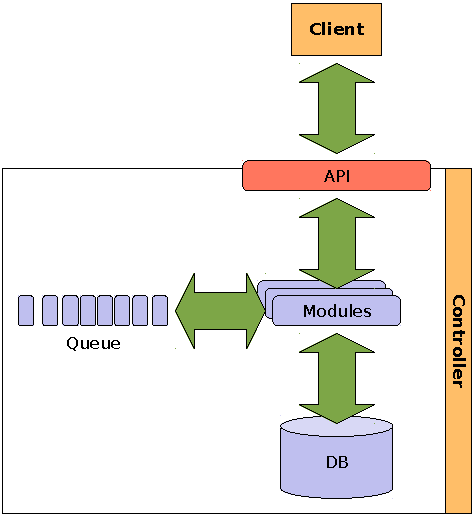
\includegraphics[width=0.5\textwidth]{imagenes/005.pdf}
 \caption{Detalle del controlador de cloud}
\label{fig:cloudcontroller}
\end{center}
\end{figure}

Normalmente, los clientes interact\'uan con el cloud a trav\'es de un API REST (\emph{REpresentational State Transfer}). Estos clientes suelen tener forma de herramienta de interfaz de comandos (\emph{CLI} o \emph{Command Line Interface}) o interfaz web, consumidoras de un servicio REST, de ah\'i que el API de acceso tenga que exponer un servicio de ese tipo. Estos APIs de acceso var\'ian li\-ge\-ra\-men\-te en sintaxis y sem\'antica con cada compa\~n\'ia, lo que provoca cierto acoplamiento de los clientes con los servicios. Es por ello que se han puesto en marcha numerosos esfuerzos para la unificaci\'on y estandarizaci\'on de estos APIs, para garantizar la compatibilidad entre distintas implementaciones, siendo el m\'as importante por primerizo y acogida, el propuesto desde el \emph{Open Grid Forum}: \emph{OCCI} (\emph{Open Cloud Computing Interface} \cite{occisdraft}).\newline

Los m\'odulos constitutivos del cloud soportan el grueso funcional del controlador. Cada uno de ellos tendr\'a un fin bien definido, y as\'i aparecen m\'odulos de red, m\'odulos de control de acceso y seguridad, m\'odulos de almacenamiento, etc. Muchos de ellos ya exist\'ian previa aparici\'on de los cloud, s\'olo que funcionaban de manera aislada. Los m\'odulos se comunican entre s\'i usando una cola de mensajes as\'incrona que garantiza la comunicaci\'on tambi\'en con el exterior del controlador, es decir, con el resto de los nodos del cl\'uster que participa en el cloud. Y por \'ultimo, la base de datos, soporte de almacenamiento de informaci\'on compartida por los m\'odulos de la nube, jugar\'a un papel central, ya que la informaci\'on global de estado determina el comportamiento general del cloud. Si estos datos se corrompiesen, el funcionamiento general podr\'ia verse gravemente afectado.\newline

Los requisitos operativos var\'ian seg\'un el framework en cuesti\'on y el tipo de servicio que se pretenda garantizar, pero generalmente, algo que se a\-pro\-xi\-me a 10 GB de RAM, cu\'adruple n\'ucleo,  \emph{Gigabit Ethernet} y alg\'un TB de almacenamiento ser\'ia m\'as que suficiente.


\subsubsection{Cloud Node}\label{subsubsec:cloudnode}

\noindent Si el controlador de la nube es quien se encarga de mantenerla funcionando haciendo de pegamento de las partes, el soporte de procesado se lo llevan los nodos. Esto es, la CPU, la memoria de ejecuci\'on y la memoria de disco de cada servidor virtual se van a tomar prestadas de las correspondientes variables CPU, RAM y disco de los anfitriones (nodos) del cl\'uster real.\newline

Los nodos del cloud pueden ser, en cierto grado, heterog\'eneos en cuanto a caracter\'isticas hardware. Ellos van a configurar un grupo de recursos que visto desde fuera ser\'a como un todo homog\'eneo, donde la suma de las capacidades de cada nodo es la dimensi\'on de la infraestructura de la nube. Adem\'as, este espacio homog\'eneo podr\'a ser provisto, como ya se ha comentado, bajo demanda. Es tarea del controlador del cloud determinar el modo \'optimo de reparto de los servidores virtuales entre los nodos, atendiendo, entre otras, a las caracter\'isticas t\'ecnicas de ambos ---nodo \emph{f\'isico} y m\'aquina virtual.\newline

El subsistema m\'as importante de los nodos del cloud es el \emph{hipervisor} o monitor de m\'aquina virtual (\emph{VMM}). Se encarga de hacer posible la ejecuci\'on de servidores virtuales (instancias) creando la arquitectura virtual necesaria y un \emph{dominio virtual de ejecuci\'on} que ser\'a manejado por el hipervisor y el kernel del sistema operativo del nodo del cloud. Para generar esta arquitectura existen fundamentalmente tres t\'ecnicas: \emph{emulaci\'on}, \emph{paravirtualizaci\'on} y \emph{virtualizaci\'on hardware} o \emph{virtualizaci\'on completa}. Los diferentes hipervisor soportar\'an en distinta medida cada una de ellas; siendo mayoritaria la implementaci\'on de una sola de esas t\'ecnicas.\newline

\subsection{T\'ecnicas de virtualizaci\'on}\label{subsec:tecnicasemu}

\noindent A continuaci\'on se har\'a un repaso conciso sobre los principales m\'etodos de virtualizaci\'on.

\subsubsection{Emulaci\'on}\label{subsubsec:emulacion}

\noindent La emulaci\'on es la t\'ecnica de virtualizaci\'on m\'as general, en sentido de que no requiere nada especial en el hardware subyacente. En contrapartida, la penalizaci\'on de rendimiento es la m\'as acusada. En la virtualizaci\'on por emu\-la\-ci\'on, todas las estructuras que sostienen la ejecuci\'on de los servidores virtuales se generan como copias software que emulan el comportamiento de sus an\'alogas hardware. Es decir, cada instrucci\'on m\'aquina que haya de ser ejecutada en la estructura emulada tendr\'a que ser traducida \emph{en el momento} a otra instrucci\'on que pueda procesar la arquitectura real. En funci\'on de la implementaci\'on del int\'erprete y de las diferencias entre hardware emulado y hardware real, aparecer\'a una siempre elevada sobrecarga que en la ma\-yo\-r\'i\-a de los casos impide que la emulaci\'on sea utilizada en entornos de alto rendimiento. Sin embargo, gracias a su flexibilidad operativa, s\'i es un buen mecanismo de soporte de arquitecturas \emph{legacy}. Adem\'as, el kernel del hu\'esped ---el kernel del sistema operativo que corre en el servidor virtual--- no precisa modificaci\'on, y el kernel del anfitri\'on s\'olo cargar un m\'odulo, normalmente.\newline

\subsubsection{Virtualizaci\'on hardware}\label{subsubsec:virthardware}

\noindent La virtualizaci\'on hardware, por contra, permite que los procesos del hu\'esped corran encima del hardware real directamente, sin necesidad de in\-ter\-me\-dia\-rios. L\'ogicamente, esto propicia una aceleraci\'on considerable con respecto a la emulaci\'on, pero impone que el hardware d\'e un trato especial a esos procesos virtuales. En el caso de la CPU, tanto las de AMD como las de Intel soportan la ejecuci\'on virtual de procesos ---o dicho de otra forma, la ejecuci\'on de procesos pertenecientes al dominio virtual con reducida penalizaci\'on al rendimiento--- siempre que est\'en presentes las extensiones convenientes (\emph{SVM} para AMD y \emph{VT-X} para Intel \cite{intelvtx}). Igual que en la emulaci\'on, no es necesario modificar el kernel del hu\'esped, lo cual es importante ya que reducir\'ia la diversidad de sistemas operativos instalables, y el kernel anfitri\'on s\'olo ha de cargar un m\'odulo, ge\-ne\-ral\-men\-te. Apuntar, por \'ultimo, que la arquitectura hardware se presenta a las m\'aquinas virtuales tal y como es, es decir, sin ninguna alteraci\'on software intermedia.\newline

\subsubsection{Paravirtualizaci\'on}\label{subsubsec:paravirt}

\noindent La paravirtualizaci\'on utiliza una aproximaci\'on diferente. Para empezar, es indispensable que el kernel hu\'esped sea modificado, de forma que sea consciente de estar corriendo en un entorno paravirtualizado. A la hora de ejecutar, el hipervisor marcar\'a aquellas regiones del c\'odigo que sean comprometidas, esto es, que deban correrse en modo kernel en la CPU, dejando al margen las partes en modo usuario que podr\'an ser ejecutadas como procesos del anfitri\'on. A continuaci\'on, el hipervisor gestionar\'a un contrato de ejecuci\'on entre el hu\'esped y el anfitri\'on, de forma que este \'ultimo procesar\'a esas partes en modo kernel como si se tratasen de secciones del dominio real de procesado, y no como pertenecientes al dominio virtual con su correspondiente penalizaci\'on de rendimiento. La paravirtualizaci\'on, en cambio, no requiere ninguna extensi\'on especial en el hardware.\newline


\subsection{Frameworks para cloud IaaS}\label{subsec:frameworksiaas}

\noindent Los frameworks para cloud IaaS son aquellos sistemas software encargados de abstraer la complejidad asociada al aprovisionamiento din\'amico y la administraci\'on de infraestructura gen\'erica susceptible de fallar. Casi en su totalidad en c\'odigo abierto bajo licencia Apache ---lo que facilita las aportaciones y la reutilizaci\'on de m\'odulos de unos a otros---, sin embargo han tenido marcos de evoluci\'on diferentes. Este hecho ha condicionado su falta de in\-te\-ro\-pe\-ra\-bi\-li\-dad hacia el exterior ---con clientes consumidores del cloud--- cuajando APIs de gesti\'on no estandarizadas; aunque hoy por hoy empieza a no ser cierto. Estos frameworks no dejan de ser producto del esfuerzo por mejorar y facilitar la administraci\'on de los clusters concretos sobre los que se fueron gestando. Por tanto, no es de extra\~nar que sus avances se hayan producido en paralelo con la infraestructura que gestionaban, sin importar demasiado la compatibilidad.\newline

Poco a poco, estos sistemas de manejo fueron creciendo en alcance y res\-pon\-sa\-bi\-li\-dad impulsados por el creciente inter\'es del sector. Al final, sucedi\'o que la propia ingenier\'ia del software y de sistemas los fue haciendo cada vez m\'as gen\'ericos, de manera que terminaron por solaparse funcionalmente. La aparici\'on de los AWS termin\'o de fraguar la necesidad latente de estandarizaci\'on, y as\'i, la mayor\'ia de estos frameworks ofrecen APIs propios cada vez m\'as pr\'oximos al de Amazon, hoy por hoy est\'andar de facto, y que adem\'as est\'an siendo remodelados para dirigirse hacia el est\'andar OCCI \cite{occisdraft}.


\section{Paradigma MapReduce}\label{sec:mapred}
\noindent El origen del paradigma se centra en el art\'iculo \cite{googlemapreduce}. En \'el se investigaba la posibilidad de abstraer las partes comunes de la utilizaci\'on de recursos computacionales distribuidos, que tanto aumentaban la complejidad de algunos problemas simples que se planteaban cotidianamente en Google. As\'i fue tomando forma la primera implementaci\'on de un modelo que se ocupaba de todos los apartados necesarios para aprovechar las capacidades de c\'alculo y almacenamiento de los clusters de que dispon\'ian. Una concisa definici\'on dicta que MapReduce es un ``\textit{modelo de procesado de datos y entorno de ejecuci\'on que corre en grandes clusters de computadores personales convencionales}'' \cite{hadoopdefguide}.


\subsection{Modelo de programaci\'on}\label{subsec:programacionmapred}
\noindent El modelo del programaci\'on del paradigma requiere que el desarrollador ex\-pre\-se su problema como un contrato de procesado en dos partes fundamentales. La primera parte se encarga de leer los datos de entrada y de producir unos resultados intermedios que ser\'an distribuidos por la red. Estos resultados intermedios se agrupar\'an seg\'un el valor de una clave intermedia. Una segunda fase comienza con los resultados intermedios agrupados y finaliza cuando se han \emph{reducido} todas las operaciones pendientes sobre las agrupaciones de entrada. Visto desde otra perspectiva, la primera fase se co\-rres\-pon\-de, a grandes rasgos, con el comportamiento de la funci\'on \emph{map} y la segunda con la funci\'on \emph{fold}; ambas pertenecientes al modelo de programaci\'on funcional. \newline

En el vocabulario del framework MapReduce, estos conceptos de la programaci\'on funcional dan origen a las funciones \texttt{Map} y \texttt{Reduce} que definen los trabajos de procesado. Tanto Map como Reduce han de ser escritas por parte del programador, lo que puede obligar a cambiar el modo de expresi\'on del problema original. A cambio, el framework se encarga de paralelizar la computaci\'on, distribuyendo los datos de entrada, manejando los errores que pudiesen producirse y recogiendo los resultados a la salida; todo de forma transparente.


\subsubsection{Funci\'on Map}\label{map}
\hyphenation{MapReduce}
\noindent El t\'ipico map funcional toma una funci\'on \emph{F} cualquiera y una lista de elementos \emph{L} o, en general, cualquier estructura recursiva, para devolver la lista resultado de aplicar \emph{F} a cada elemento de \emph{L}. La figura \ref{fig:functionalmap} muestra su firma y un ejemplo de aplicaci\'on.\newline

\begin{figure}[tbp]
\begin{center}
\begin{tabular}{|l|}
\hline
$\mathbf{map:} \: \left ( \alpha \rightarrow \beta \right ) \: \rightarrow \: \alpha \: list \: \rightarrow \: \beta \: list$ \\
$\mathbf{map} \: \left( \mathbf{pow}\:2 \right) \: \left[ 1,2,3 \right] \: \Rightarrow \: \left[ 1,4,9 \right ]$ \\
\hline
\end{tabular}
\caption{Ejemplo de aplicaci\'on de la funci\'on map (versi\'on funcional)}
\label{fig:functionalmap}
\end{center}
\end{figure}

En su realizaci\'on MapReduce, la funci\'on Map recibe un par de valores a la entrada y produce otro par \texttt{(clave, valor)} como salida intermedia. La librer\'ia MapReduce se encarga entonces de agrupar esos pares intermedios, por valor de clave, antes de pas\'arselos a Reduce como entradas. Los tipos de entrada y salida de Map se corresponden con la firma de la figura \ref{fig:mapreducemap}. Es el framework MapReduce quien se encarga de alimentar la funci\'on Map, transformando los datos de los ficheros de entrada en pares \texttt{(clave, valor)} correctos.

\begin{figure}[tbp]
\begin{center}
\begin{tabular}{|l|}
\hline
$\mathbf{map:} \: \left( k1,v1 \right) \: \rightarrow \: \left( k2,v2 \right) list$ \\
$\mathbf{k:} \: clave \linebreak$ \\
$\mathbf{v:} \: valor \linebreak$ \\
$\mathbf{\left(kn,vn \right):} \: par \: \left( clave,valor \right) \: en \: un \: dominio \: n$ \\
\hline
\end{tabular}
\caption{Firma de la funci\'on Map (versi\'on MapReduce)}
\label{fig:mapreducemap}
\end{center}
\end{figure}


\subsubsection{Funci\'on Reduce}\label{reduce}
\noindent El t\'ipico fold de la programaci\'on funcional recoge una funci\'on \emph{G} cualquiera, una lista \emph{L}, gen\'ericamente cualquier estructura recursiva, y un elemento inicial \emph{I}, del mismo tipo que los elementos de \emph{L} y sobre el que se acumulan los resultados intermedios, para devolver el valor final de \emph{I}, resultado de aplicar \emph{G} a cada elemento de \emph{L}. La figura \ref{fig:fold} presenta su firma y un ejemplo de aplicaci\'on.\newline

\begin{figure}[tbp]
\begin{center}
\begin{tabular}{|l|}
\hline
$\mathbf{fold:} \: \left( \alpha \rightarrow \beta \rightarrow \alpha \right) \: \rightarrow \: \alpha \: \rightarrow \: \beta \: list \: \rightarrow \: \alpha$ \\
$\mathbf{fold} \: \left( \mathbf{+} \right) \: 0 \: \left[ 1,2,3 \right] \: \Rightarrow \: 6$ \\
\hline
\end{tabular}
\caption{Ejemplo de aplicaci\'on de la funci\'on fold}
\label{fig:fold}
\end{center}
\end{figure}

A la funci\'on Reduce, en cambio, se le pasan las agrupaciones intermedias formadas por una clave y su conjunto de valores asociado, la salida de Map, para producir en su salida un conjunto menor de valores, ya que cada invocaci\'on de Reduce ocasionar\'a cero o un \'unico valor por cada clave, \emph{reduciendo} o plegando (fold) esos valores intermedios. La firma de Reduce se presenta en la figura \ref{fig:reduce}. Del mismo modo a como sucede en Map, es el framework quien se encarga de gestionar la transferencia de los resultados intermedios, salida de Map, a Reduce. A este respecto decir que algunas implementaciones del modelo permiten al desarrollador controlar el modo en que gestionan los resultados intermedios, pudiendo definir el comportamiento de las agrupaciones en una funci\'on \texttt{Combiner} que act\'ua antes de Reduce.

\begin{figure}[tbp]
\begin{center}
\begin{tabular}{|l|}
\hline
$\mathbf{reduce:} \: \left( k2,v2 \: list \right) \: \rightarrow \: v2 \: list$ \\
$\mathbf{k:} \: clave$ \\
$\mathbf{v:} \: valor$ \\
$\mathbf{\left(kn,vn \right):} \: par \: \left(clave,valor\right) \: en \: un \: dominio \: n$ \\
\hline
\end{tabular}
\caption{Firma de la funci\'on Reduce}
\label{fig:reduce}
\end{center}
\end{figure}


\subsubsection{Wordcount en MapReduce}\label{subsubsec:wordcount}
\noindent Como ejemplo, la figura \ref{fig:wordcount} contiene el pseudoc\'odigo de una aplicaci\'on MapReduce para contar el n\'umero de apariciones de distintas palabras en una serie de documentos.\newline

\begin{figure}[tbp]
 \begin{center}
  \begin{tabular}{|l|}
   \hline
   \texttt{{\bf Map} (String key, String value):} \\
   \texttt{// key: nombre del documento} \\
   \texttt{// value: contenido del documento} \\
   \texttt{{\bf for each} word w {\bf in} value:} \\
   \texttt{{\bf EmitIntermediate} (w, ``1'')};\\ \\

   \texttt{{\bf Reduce} (String key, Iterator values):} \\
   \texttt{// key: una palabra} \\
   \texttt{// values: un iterable sobre un n\'umero de palabras} \\
   \texttt{{\bf int} result = 0;} \\
   \texttt{{\bf for each} v {\bf in} values:} \\
   \texttt{{\bf Emit} ({\bf AsString} (result));} \\
   \hline
  \end{tabular}
  \caption{Pseudoc\'odigo de wordcount para MapReduce. Fuente: \cite{googlemapreduce}}
  \label{fig:wordcount}
 \end{center}
\end{figure}

En una ejecuci\'on de \texttt{wordcount} suceder\'a lo siguiente: a la entrada de Map se situar\'an tanto el nombre de cada documento como su contenido en texto plano. Map recorrer\'a entonces cada documento al completo emitiendo el par \texttt{(<palabra>, ``1'')} por cada palabra de cada documento. De este modo, se producir\'a una explosi\'on de pares intermedios que representan ya la soluci\'on del problema; s\'olo resta agrupar los pares por palabra y sumar el n\'umero de ocurrencias de cada par ---la funci\'on Reduce. Al Reduce de \texttt{wordcount} se le presentar\'a, por cada palabra de cada documento, la lista, o en general el \emph{iterable}, que contenga todos los valores asociados a esa palabra, es decir, una lista con tantos \texttt{``1''} como veces haya aparecido la palabra en todos los documentos. Al concluir la ejecuci\'on, MapReduce devolver\'a un listado con todas las palabras visitadas y el n\'umero de veces que aparece cada una de ellas.


\subsection{Aplicabilidad del modelo}\label{subsec:aplicabilidad}
\noindent La diversidad de problemas que pueden expresarse usando este paradigma aparece reflejado en \cite{googlemapreduce}, por ejemplo:
\begin{itemize}
 \item Grep distribuido: map emite cada l\'inea que concuerde con el patr\'on introducido. Reduce s\'olo copia sus entradas a la salida (funci\'on \emph{identidad}).
 \item Recuento de la frecuencia de acceso a un URL: muy parecido al wordcount.
 \item Gr\'afico inverso web-enlace: para cada URL destino contenido en una web origen, Map genera el par \texttt{(<URLdestino>, <URLorigen>)}
 \item \'Indice invertido: Map parsea cada documento y emite una serie de pares de la forma \texttt{(<palabra>, <iddocumento>)}. Todos ellos son pasados como entrada a Reduce que elabora la secuencia de pares \texttt{(<palabra>, list(iddocumento)}).
\end{itemize}



\subsection{Modelo de procesado}\label{subsec:processingmodel}
\noindent Adem\'as de definir la estructura que han de seguir los programas que quieran apoyarse en la librer\'ia MapReduce, en vez de escribir sus propios me\-ca\-nis\-mos para el empleo de computaci\'on distribuida, con \cite{googlemapreduce} se propuso una implementaci\'on del modelo que permitiese mejorar el modo de utilizaci\'on de los recursos computacionales de que dispon\'ian en Google:

\begin{itemize}
 \item Linux, doble procesador, 2-4 GB de RAM.
 \item 100 Mb/s \'o 1 Gb/s de ancho de banda de red en las m\'aquinas.
 \item Cientos o miles de m\'aquinas por cl\'uster, es decir, se producir\'an fa\-llos de ejecuci\'on ineludiblemente.
 \item Discos duros IDE y sistema de ficheros distribuido manejando la informaci\'on en ellos.
\end{itemize}

As\'i evitamos el uso de protocolos, arquitecturas, sistemas operativos o software de comunicaci\'on propietarios: ideal para despliegues gen\'ericos.\newline

Cada petici\'on de ejecuci\'on MapReduce se denomina \emph{trabajo}. Cada trabajo est\'a compuesto por m\'ultiples \emph{tareas}. La finalizaci\'on de un trabajo requiere la conclusi\'on del procesamiento de todas las tareas. La m\'axima del modelo de procesado es paralelizar la ejecuci\'on de las tareas en cada nodo participante. De forma general, se puede afirmar que las tareas de cada fase ---las tareas de la fase Map y las de la fase Reduce--- se procesan en paralelo y que las fases se suceden en serie. Sin embargo, no es necesario que haya terminado \emph{completamente} la fase Map para que comience la Reduce.\newline

La figura \ref{fig:exmapreduce} muestra un resumen del flujo de ejecuci\'on t\'ipico de procesado MapReduce. Es interesante describirlo ya que los distintos frameworks que se adhieren al modelo MapReduce van a presentar aproximaciones muy similares.

\begin{figure}[tbp]
\begin{center}
 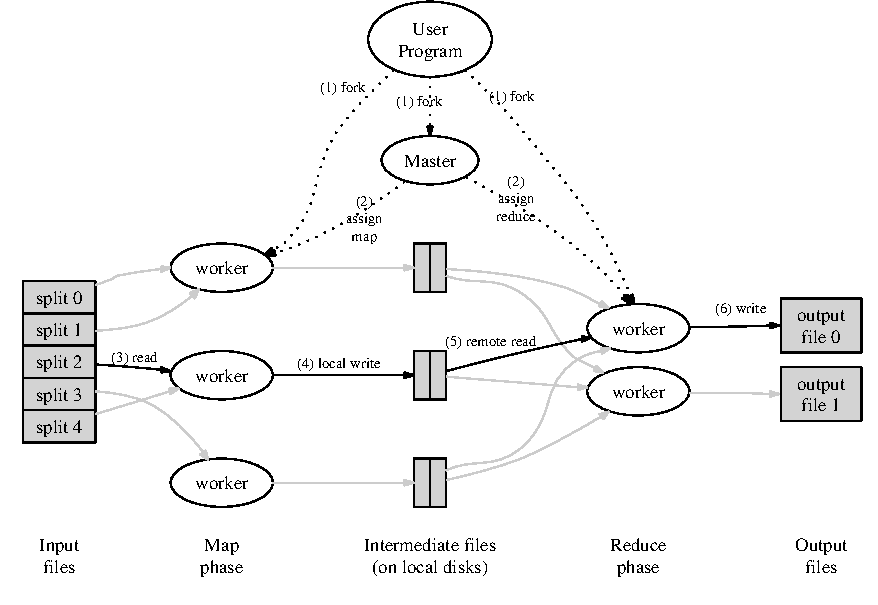
\includegraphics[width=0.9\textwidth]{imagenes/006.pdf}
 \caption{Diagrama de ejecuci\'on MapReduce. Fuente: \cite{googlemapreduce}}
 \label{fig:exmapreduce}
\end{center}
\end{figure}


\begin{enumerate}
 \item MapReduce divide los ficheros de entrada en \emph{M} partes, de tama\~no configurable usando un par\'ametro, y distribuye tantas copias del programa del usuario ---t\'ipicamente s\'olo las implementaciones concretas de Map y Reduce--- como nodos participen en la computaci\'on.
 \item Ahora cada copia del programa reside en un nodo. Se define entonces que una de esas copias sea especial ---la r\'eplica \emph{Master}--- de forma que el resto quedan residiendo en nodos que, en adelante, son considerados \emph{trabajadores} o \emph{esclavos}. O dicho de otro modo, desde el momento en que se nombra la copia maestra, se determina el rol \emph{maestro} del cl\'uster, que recae sobre el nodo que posee la copia maestra; los dem\'as nodos tendr\'an en su poder copias no maestras o esclavas, fijando, igualmente, su rol a esclavos. Estos nodos esclavos son los que reciben las tareas concretas de ejecuci\'on dirigidos por el maestro. Habr\'a \emph{M} tareas Map y \emph{R} tareas Reduce que el maestro ha de repartir entre sus trabajadores inactivos y que podr\'an ser procesadas en paralelo.
 \item Los trabajadores a los que se les hayan asignado tareas Map leen las porciones de los ficheros de entrada correspondientes, \emph{parsean} los do\-cu\-men\-tos generando pares \texttt{(clave, valor)} que redirigen a la funci\'on Map del usuario. El contenido de salida de Map se mantiene en memoria a modo de b\'uffer.
 \item Peri\'odicamente, esos pares en memoria son volcados a \emph{disco local} y particionados en \emph{R} regiones. Su posici\'on en disco es enviada al maestro, responsable de informar de la localizaci\'on de esos pares intermedios a los trabajadores con tareas Reduce.
 \item En el momento en que un trabajador Reduce es notificado de que sus datos de ejecuci\'on, esto es, los datos de una partici\'on que le co\-rres\-pon\-de, est\'an disponibles, \'este lee la informaci\'on del disco del trabajador Map a trav\'es de \emph{RPC} (\emph{Remote Procedure Call}) y, antes de invocar la funci\'on Reduce del usuario, ordena los pares intermedios por clave.
 \item Finalmente, el trabajador Reduce itera sobre los pares ordenados por clave, enviando, a la funci\'on Reduce del usuario, la clave y el conjunto de valores asociados a esa clave. La salida de la funci\'on Reduce para esa partici\'on se va escribiendo en un archivo de salida sobre el sistema de ficheros distribuido.
\end{enumerate}

Cuando se hayan completado todas las tareas Map y Reduce, el espacio particionado de salida ---los ficheros de salida de cada partici\'on--- se env\'ia al programa que haya hecho la llamada a MapReduce.
El modelo de ejecuci\'on es lo suficientemente gen\'erico como para aplicarse a la resoluci\'on de problemas de distinto tama\~no, corriendo sobre clusters indeterminadamente grandes.


\subsection{Tolerancia a fallo}\label{subsec:toleranciafallos}
\noindent La idea de proporcionar un marco de ejecuci\'on de trabajos lo suficientemente grandes como para necesitar enormes conjuntos de m\'aquinas de procesado para mantener los tiempos de latencia en valores razonables, pasa, forzosamente, por definir una pol\'itica que asegure cierta resistencia a unos fallos que seguramente aparecer\'an. De no ser considerados, estos fallos derivar\'ian en errores de distinto grado de severidad: unos provocar\'ian que se perdiesen tareas ya completadas, otros, menos problem\'aticos, inhibir\'ian los datos intermedios, siendo improbable la conclusi\'on con \'exito de la ejecuci\'on. Sea como fuere, el propio modelo MapReduce prevee una serie de problemas en el procesamiento e implementa una serie de actuaciones ante cada uno de ellos.


\subsubsection{Fallo en trabajador}\label{subsubsec:fallotrabajador}
\noindent El menos problem\'atico. Para controlar que todos los trabajadores al cargo de un maestro funcionan correctamente, cada cierto tiempo el maestro env\'ia una petici\'on de respuesta de eco ---el cl\'asico \emph{ping}--- a todos estos trabajadores. Si alguno de ellos no contestase de forma reiterada, \'este quedar\'ia registrado en el maestro como \emph{inaccesible}.\newline

Un trabajador marcado inaccesible no recibir\'a nuevas tareas, ni tampoco podr\'a ser accedido remotamente por los trabajadores Reduce para cargar los resultados de sus Map intermedios, lo que puede suponer un problema insalvable para completar la ejecuci\'on. El acceso a estos datos intermedios se resuelve marcando, de nuevo en el maestro, las tareas asignadas al trabajador ca\'ido como \emph{inactivas}. As\'i, \'estas ser\'an programadas para ser procesadas de nuevo en alg\'un trabajador activo, que colocar\'a los resultados intermedios en alg\'un punto accesible por los nodos Reduce. Adem\'as, en el momento de detectar la incapacidad operativa de un trabajador, el maestro informar\'a de este hecho al resto de trabajadores esclavos para evitar, por ejemplo, errores en la lectura de los datos intermedios.


\subsubsection{Fallo en maestro}\label{subsubsec:fallomaestro}
\noindent El fallo en el nodo maestro es el m\'as problem\'atico. La aproximaci\'on propuesta consiste en ordenar que el maestro cree peri\'odicamente puntos de restauraci\'on desde los que pueda reanudar su ejecuci\'on en caso de que se terminase inesperadamente. Ya que el maestro es \'unico, la probabilidad de fallo es mucho menor que para el caso general de fallo en un nodo; de hecho, lo suficientemente baja como para que se proponga en \cite{googlemapreduce} que se aborte la ejecuci\'on del trabajo al completo si el maestro fallase. Como primera soluci\'on es acep\-ta\-ble. No obstante, dado que no tiene ning\'un sentido dejar un \emph{punto de fallo singular} f\'acil de abordar al descubierto, frameworks posteriores proponen replicar el comportamiento del maestro en otros nodos.


\subsection{Caracter\'isticas adicionales}\label{subsec:caracteristicasadicionales}
\noindent A continuaci\'on se resumen otras cuestiones adicionales estudiadas para este framework MapReduce.

\subsubsection{Localidad}\label{subsubsec:localidad}
\noindent El cuello de botella en un despliegue t\'ipico es el ancho de banda de red. En una ejecuci\'on cualquiera, la informaci\'on se propaga desde el cliente hacia el sistema de ficheros distribuido del cl\'uster MapReduce. Como se ha comentado, cada nodo posee una cierta capacidad de almacenamiento y ejecuci\'on de tareas sobre los datos de entrada. De esta forma, cada paso del procesado global requiere la transmisi\'on por la red de enormes cantidades de informaci\'on ---recordar, por ejemplo, la E/S de la funci\'on Map en wordcount--- colapsando r\'apidamente su ancho de banda y limitando, por tanto, la velocidad de ejecuci\'on. Para mitigar este problema, se afina el sistema de ficheros distribuido para que aproxime la informaci\'on al nodo del cl\'uster que ha de procesar esa informaci\'on, reduciendo considerablemente las transferencias acometidas para completar los trabajos, minimizando as\'i el tr\'afico de red requerido.


\subsubsection{Complejidad}\label{subsubsec:complejidad}
\noindent A priori, las variables \emph{M} y \emph{R} de las ejecuciones MapReduce ---recordemos, la dimensi\'on de las particiones del espacio de entrada e intermedio res\-pec\-ti\-va\-men\-te--- pueden tomar valores cualesquiera configurables por el usuario. Sin embargo, existen ciertos l\'imites pr\'acticos. Por cada trabajo MapReduce que se est\'e gestionando, el maestro ha de hacer $O(M + R)$ decisiones de planificaci\'on ---suponiendo que no se produjese ning\'un error que forzase replanificar tareas--- ya que cada partici\'on del espacio de entrada, \emph{M}, habr\'a de repartirse entre los trabajadores Map, y cada partici\'on del espacio de salida de Map, \emph{R}, entre los trabajadores Reduce; de ah\'i la expresi\'on de la \emph{complejidad temporal}. En cuanto a la \emph{complejidad espacial}, el maestro tendr\'a que mantener $O(M \cdot R)$ de memoria de estado. La expresi\'on se optiene al razonar que, en el peor de los casos, cada parte del fichero de entrada se mapear\'a sobre cada parte del espacio intermedio.


\subsubsection{Tareas secundarias}\label{subsubsec:secundarias}
\noindent Podr\'ia caber la situaci\'on en la que un nodo del cl\'uster estuviese ejecutando tareas Map o Reduce a una velocidad m\'as lenta de lo habitual; por ejemplo, si tuviese el disco r\'igido da\~nado, las lecturas y escrituras se suceder\'ian m\'as lentamente, y como el trabajo MapReduce no est\'a completado hasta que todas sus tareas componentes hayan finalizado con \'exito, el nodo problem\'atico estar\'ia ocasionando una limitaci\'on en el rendimiento global. Para aliviar el problema, se propone que cuando falte por concluir la ejecuci\'on de pocas ta\-re\-as del trabajo, \'estas sean enviadas a dos nodos trabajadores: una como tarea convencional y otra como tarea secundaria de alg\'un nodo inactivo. En el momento en que concluya la ejecuci\'on de alguna de las dos, esa tarea se marcar\'a como terminada, reduciendo la latencia que a\~naden esos nodos con dificultades operativas.


\subsubsection{Funci\'on Combiner}\label{subsubsec:combiner}
\noindent En muchas ocasiones sucede que existe un gran n\'umero de pares intermedios generados que se repiten. Tomando como ejemplo el wordcount expuesto antes, se puede deducir que cada trabajador Map generar\'a ingentes cantidades de registros de la forma \texttt{(``a'', ``1'')}, que ser\'an enviados por la red hacia los trabajadores Reduce. Un mecanismo para reducir este colapso es permitir al usuario escribir una funci\'on de combinaci\'on de resultados intermedios, que se lanzar\'a previa ejecuci\'on de la funci\'on Reduce. Esta funci\'on combinadora ir\'a recogiendo los resultados intermedios, dentro del mismo trabajador Map, para hacer una primera reducci\'on (o combinaci\'on) de los datos antes de ser marcados como disponibles para los trabajadores Reduce.\newline

T\'ipicamente, el c\'odigo fuente de ambas funciones ---Reduce y Combiner--- es el mismo; lo que s\'i cambia es el modo en que la librer\'ia MapReduce gestiona su ejecuci\'on: la salida de la combinaci\'on se mantiene en disco local y no en el sistema de ficheros distribuido, para reducir la sobrecarga de red que supondr\'ia.


\subsection{Frameworks MapReduce}\label{subsec:frameworksmapred}
\noindent Desde 2004 han ido apareciendo multitud de frameworks que codifican, considerando distintas optimizaciones, la funcionalidad del paradigma. Por citar algunos nombres:

\begin{description}
 \item[Hadoop] \cite{hadoopdefguide} Uno de los primeros en cubrir el modelo de procesado pro\-pues\-to para MapReduce y principal implementaci\'on de referencia para los dem\'as frameworks. Es el m\'as utilizado, probado y desplegado con diferencia en la actualidad.
 \item[GridGain] \cite{gridgainvshadoop} Comercial y centrado en el procesado en memoria para ace\-le\-rar la ejecuci\'on: menor latencia de acceso al dato a costa de un menor espacio de E/S.
 \item[Twister] \cite{twister} Desarrollado como proyecto de investigaci\'on en la Universidad de Indiana, pretende dar un giro de tuerca m\'as al modelo MapReduce, abstrayendo las partes comunes y necesarias para lanzar ejecuciones, aisl\'andolas y almacen\'andolas en memoria distribuida como objetos est\'aticos, reduciendo as\'i el tiempo necesario para configurar las funciones Map y Reduce previo procesado.
 \item[GATK] \cite{gatk} Utilizado en investifaci\'on gen\'etica para evaluar y secuenciar fragmentos de ADN de m\'ultiples especies.
 \item[Qizmt] \cite{qizmt} Escrito en C\# y puesto en funcionamiento para MySpace.
 \item[misco] \cite{misco} Escrito 100\% en Python y basado en trabajos previos de Nokia, se propone como implementaci\'on MapReduce capaz de correr en dispositivos m\'oviles.
 \item[Peregrine] \cite{peregrine} Optimizando el modo en que se manipulan los resultados intermedios y pasando toda operaci\'on de E/S a una cola as\'incrona, entre otras alteraciones, han llegado a acelerar bastante la ejecuci\'on de tareas. Todav\'ia en beta a junio de 2013.
 \item[Mars] \cite{mars} Implementado en \emph{NVIDIA CUDA}, se centra en extraer el m\'aximo rendimiento de mapeo y reducci\'on moviendo la operativa a la tarjeta gr\'afica. En seis pruebas realizadas con Mars se han observado incrementos de rendimiento superiores a un orden de magnitud frente a ejecuciones en CPU.

\end{description}

De todos ellos Hadoop es, incuestionablemente, el framework MapReduce m\'as utilizado en la actualidad. Su naturaleza de c\'odigo abierto y su flexibilidad, tanto de procesado como de almacenamiento, le han reportado un creciente inter\'es desde la industria de la IT, que se ha venido traduciendo en la aparici\'on de numerosas herramientas acoplables a Hadoop que extienden su funcionalidad.


